\chapter{Conceptual Design}
\label{ch:conceptualDesign}

\section{Requirements}
\label{ch:requirements}

In a first step, requirements towards the synthetic data generation system will be established.
The goal is to gather a systematic collection of requirements on which the success of the developed system can be meassured.
Firstly, non-functional requirements will be explained and secondly, the functional requirements will be explained.


\subsection*{Non-Functional Requirements}

Non-functional requirements (or qualitative requirements) describe requirements and constraints on a system that govern the manner in which the functions specified in the functional requirements are to be performed \cite{broy2021EinfuehrungSoftwaretechnik}.
They focus on the question of how a systems functional requirements should be realized \cite{broy2021EinfuehrungSoftwaretechnik}.
The ISO-Norm 25010 \cite{SystemsSoftwareEngineering} defined the base characteristics that are of relevance for a software systems quality \cite{haoues2017GuidelineSoftwareArchitecture}.
These are \cite{haoues2017GuidelineSoftwareArchitecture}:
\begin{itemize}
    \item Functional Suitability
    \item Reliability
    \item Performance efficiency
    \item Compatibility
    \item Usability
    \item Security
    \item Maintainability
    \item Portability
\end{itemize}

of which each is of difference importance for each software system.
Additionally, \cite{vogelsang2019RequirementsEngineeringMachine} highlights, that in the context of machine learning tasks, additional quality requirements might be necessary, for which a standard has yet to be defined.
These could include (but is not limited to):

\begin{itemize}
    \item Quantitative targets
    \item Explainability
    \item Freedom from Discrimination
    \item Legal and Regulatory Requirements
    \item Data Requirements
\end{itemize}

Since the focus of this thesis is rather a research prototype, than a fully developed software system, only a subset of above mentioned requirements are prioritized during development.
The following requirements R1 - RN are the non-functional requirements for the software developed in this thesis:

[TODO: GANZER ABSCHNITT AM ENDE AUF INHALTLICHE RICHTIGKEIT KORRIGIEREN]
\begin{description}
    \item[R1 - Functional Suitability:]
    Functional Suitability refers to "the degree to which a product or system provides functions that meet stated and implied needs when used under specified conditions" \cite[p. 219]{bass2013SoftwareArchitecturePractice}.
    In the context of this thesis, the system needs to be able to show how different tabular processing techniques influence the performance of an existing synthesization approach [TODO: Später nochmal überarbeiten]

    \item[R2 - Maintainability]:
    Maintainability focuses on the "degree of effectiveness and efficiency with which a product or system can be modified by the intended maintainers" \cite[p. 220]{bass2013SoftwareArchitecturePractice}
    One of the core questions of this thesis is to compare different tabular processing techniques in diffusion models.
    For this, a variety of different approaches are intended to be compared.
    Hence, it is required that the code is written in an easy maintainable way, such that it can be easily extended with additional processing techniques, not only by the developer, 
    but also for future researchers who might build upon the work of this thesis.

    \item[R3 - Performance efficiency]:
    In the context of a deep learning, the performance of the program is always of importance, since training, hyperparameter search and inference usually demand a lot of computation time by nature.
    As a consequence, the developed software should try to reduce unnecessary computations as much as possible.

    \item[R4 - Portability/Reproducibility]:
    Portability is usually referring to the extend of "effectiveness and efficiency with which a system, product, or component can be transferred from one hardware, software, 
    or other operational or usage environment to another" \cite[p. 220]{bass2013SoftwareArchitecturePractice}.
    Since this thesis should encourage other researchers to reproduce and extend the produced codebase, the software should be able to run on other machines running a different operating system given a specified development environment,
    including packages used and their version numbers.
    In general, it is required, that all results should be fully reproducible, given the parameters and the configuration of the experiment setups

    \item[R5 - Quantitative Targets]:
    It is required that the different model versions produced in the thesis are compared using metrices that are commonly used in the domain of tabular data synthesis.
    This should enhance the comparability to other approaches.
\end{description}


\subsection*{Functional Requirements}
\label{sec:func_requirements}
Functional requirements describe what the software system should do and which functional aspects need to be implemented for this.

\begin{description}
    \item[FR[TODO] - Parameter selection] 
    \item[Training Configuration]: %- device, preprocessing, seeds
    Each experiment needs a training configuration.

    \item[FR[TODO] - Training, Sampling, Evaluation[TODO:???]]  
    

    \item[FR[TODO] - Hyperparameter search]:
    In order to find the best parameters, some form of hyperparameter search should be implemented.

    \item[FR[TODO] - Adding Tabular processing]:
    An interface on tabular processing mechanisms is required, such that different mechanism can be added easily and consistently.
    
    \item[FR[TODO] - Tabular processing selection]:
    It should be possible to easily select which tabular processing mechanism will be applied

    \item[FR[TODO] - Tabular processing fit]:
    If necessary, Tabular processing mechanism should be able to be fitted.
    However, it is required, that the tabular processing mechanism only receives training data and does not have access to the test data.

    \item[FR[TODO] - Tabular processing transform]:
    Each Tabular processing mechanism needs to transform the raw data into a specified format.

    \item[FR[TODO] - Tabular processing inverse transform]:
    Each Tabular processing mechanism needs to able to inverse transformed data back into its original form.

\end{description}




% Ähnlich wie bei Masterarbeit "Generierung einer synthetischen Datenhistorie aus einem Datenbank Snapshot"
% Basierent auf ISO 2510 
% Nicht Funktional: Functional Suitability, Maintainability, (Compatibility (reproducability))

% Funktional (ergeben sich aus den Research Questions):
% - Comparability & reproducability (codebase must be able to reproduce existing results)
% - "Special Processing": must be able to handle tabular data as explained in chapter xy
% - "Special Processing": can have multiple versions (bayesian, embedding, etc.) 
% - "Special Processing": different versions should be switchable easily
% - "Special Processing": Provide general framework for possible future special processing types
% - Evaluation: must be able to evaluate the results with statistical similarity measures

- gans struggled with generating discrete variables \cite{torfi2020CorGANCorrelationCapturingConvolutionala}
- remarkable performance generating syntehtic images and time series data \cite{mckeever2020SynthesisingTabularDatasets}
- struggle with mode collapse --> generate same sample \cite{torfi2020CorGANCorrelationCapturingConvolutionala}

\section{Existing Code Base}
\label{ch:conceptualDesign-existingCodeBase}

The code \cite{akim2023TabDDPMModellingTabular} used in this experiment is based upon the work of \cite{kotelnikov2022TabDDPMModellingTabular}.
It is changed and modified according to the needs of the experiment. 
This section will firstly explain the architecture of the existing code base, before introducing the proposed adaptations in the next section.
An overview on how the overall process in this synthetic data generation approach is done, can be seen in \autoref{fig:overall_original}:


\begin{figure}[h]
    \centering
    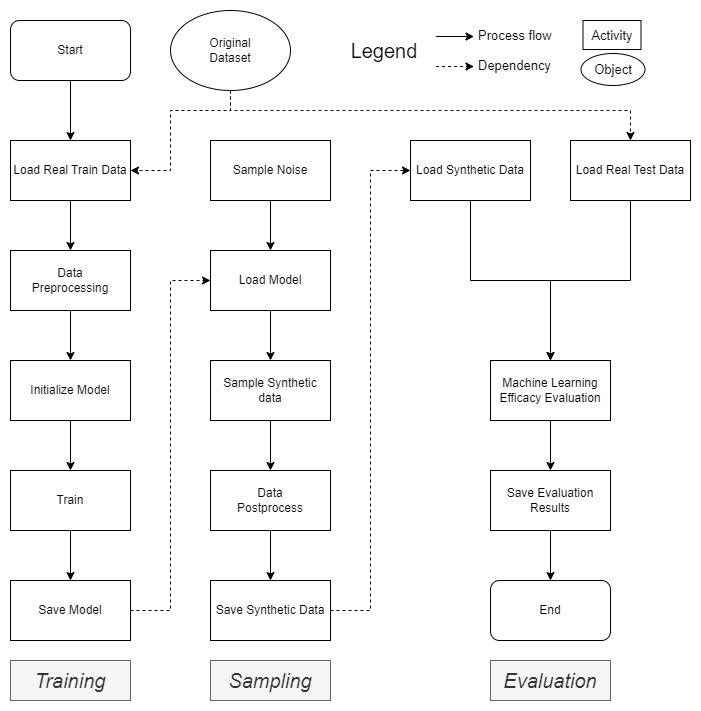
\includegraphics[width=0.8\textwidth]{images/Overall_original.png}
    \caption{Overview synthetic data generation process in \cite{akim2023TabDDPMModellingTabular}}
    \label{fig:overall_original}
\end{figure}


\subsection{Original Implementation}
\label{ch:conceptualDesign-existingCodeBase-originalImplementation}
% Why did I choose to use the existing code base?
% What are the advantages and disadvantages of the existing code base?
% Diagram explaining the current Software architecture

\subsubsection[]{Scripts}
\label{ch:scripts}

The implementation \cite{kotelnikov2022TabDDPMModellingTabular} already provides necessary scripts that allow for an
easy training, sampling, evaluation and hyperparameter tuning for their proposed TabDDPM model as well as for the models TabDDPM is compared against.
The function of the most important scripts can be summarized in the following way:

\begin{description}
    \item[train.py:]
    Does the training of the diffusion model.
    Receives configuration parameters for the training.
    Starts by loading the selected dataset and perform preprocessing according to the configuration.
    Afterwards, initializes the required class instances and starts the training loop.
    After the training loop has finished, the trained model is saved as well as its loss history.

    \item[sample.py:]
    Samples from a pre-trained diffusion model.
    Receives configuration parameters for the sampling process.
    Loads a pre-trained model and samples from the model.
    The new samples are transformed according to the inverse of the preprocessing, specified in the config.
    After transformation, the generated samples are saved.

    \item[eval\_*.py:]
    Evaluates a synthetic dataset using the machine learning efficacy.
    A machine learning model is trained on real of synthetic data, specified in the configuration.
    The performance of the model is evaluated on the real test set and metric scores are calculated.

    \item[pipeline\_*.py:]
    Defines the complete pipeline, consisting of training, sampling and evaluation.
    Handles that each function of the pipeline receives the correct attributes from the configuration.
    Allows to execute only specified parts of the pipeline individually.

    \item[tune\_*.py:]
    Responsible for the hyperparameter tuning process.
    Starts by defining a hyperparameter search space (see \cite[Table 1, p. 4]{kotelnikov2022TabDDPMModellingTabular} and \cite[Table 7-11, p. 13 f.]{kotelnikov2022TabDDPMModellingTabular})
    Next an objective function is defined, that is maximized for 50 trials through the Optuna framework \cite{optuna_2019}.
    Within the objective function, a set of hyperparameters is selected from the search space.
    With this set of hyperparameters, pipeline.py is called to train the model.
    Afterwards, for five different random initializations, pipeline.py is called to sample and evaluate the model, basically creating and evaluating five different synthetic dataset versions, produced by the model.
    In each training, sampling and evaluation, the training and validation set are redistributed and shuffled to implement some form of cross-validation \cite{kohavi2001StudyCrossValidationBootstrap}.
    The average evaluation score of the five synthetic dataset versions is returned as the objective, that Optuna tries to maximize.
    After optimization, the best hyperparameter configuration is saved.
    If specified, an final evaluation of the best found model can be started by calling eval\_seeds.py.

    \item[eval\_seeds.py:]
    Performs an extensive evaluation, given a trained model.
    Starts by loading a pre-trained sampling model ([TabDDPM|SMOTE|CTABGAN|CTABGAN+|TVAE]).
    Depending on the specified evaluation parameters, the script will produce $n_datasets$ synthetic datasets by calling the sampling script in
    pipeline\_*.py (the version of pipeline\_*.py depends on the sampling model selected).
    For each produced datasets, evaluation is performed using a predefined evaluation model ([Catboost|MLP]) for a predefined number of random initializations.
    Ultimately, the average metrics is calculated over all performed runs, reported and saved.
\end{description}

Hence, to get a fully optimized diffusion model with an extensive evaluation, the user just has tu run the tune\_ddpm.py with the --eval\_seeds flag.
A detailed activity diagram for each script can be found at [TODO: EINFÜGEN].

\subsubsection[]{Configuration}

In order to start one of the above scripts, a configuration file has to be specified, specifying the most important parameters for training, sampling and evaluation.
For example, \autoref{lst:configuration} shows how such a configuration file could look like and which parameters need to be specified

\begin{lstlisting}[label={lst:configuration}, caption={Example configuration file}]
    parent_dir = "exp/adult/check"
    real_data_path = "data/adult/"
    num_numerical_features = 6
    model_type = "mlp"
    seed = 0
    device = "cuda:0"

    [model_params]
    num_classes = 2
    is_y_cond = true

    [model_params.rtdl_params]
    d_layers = [
        256,
        256,
    ]
    dropout = 0.0

    [diffusion_params]
    num_timesteps = 1000
    gaussian_loss_type = "mse"
    scheduler = "cosine"

    [train.main]
    steps = 1000
    lr = 0.001
    weight_decay = 1e-05
    batch_size = 4096

    [train.T]
    seed = 0
    normalization = "quantile"
    num_nan_policy = "__none__"
    cat_nan_policy = "__none__"
    cat_min_frequency = "__none__"
    cat_encoding = "__none__"
    y_policy = "default"

    [sample]
    num_samples = 216000
    batch_size = 10000
    seed = 0

    [eval.type]
    eval_model = "catboost"
    eval_type = "synthetic"

    [eval.T]
    seed = 0
    normalization = "__none__"
    num_nan_policy = "__none__"
    cat_nan_policy = "__none__"
    cat_min_frequency = "__none__"
    cat_encoding = "__none__"
    y_policy = "default"

\end{lstlisting}    


Model\_type refers to the model, that should approximate the noise in the reverse noising process.
Most of the parameters are self explanatory, controlling one specific part in the whole pipeline.
For example, all model\_params specify different aspects that are relevant for instantiating the model and diffusion\_params control how the diffusion process is done.
Noteworthy are the train.T and eval.T parameters, who define how the preprocessing is done in at the beginning of training and evaluation respectively.
This configuration structure allows to easily perform a variety of experiments with different set of parameters by simply changing the configuration file and input it into the next experiment run.

\subsubsection[]{Data format}
\label{sec:data_format}
The authors provide access to 12 different dataset, which have been cleaned and formatted by a program provided by \cite[]{gorishniy2023EmbeddingsNumericalFeatures}.
Each dataset contains the data separated into multiple subparts.
Firstly, the columns are split into categorical, numerical and target ("y") columns.
Secondly, the datasets are distributed into a training, validation and testing set.
Therefore, each dataset is separated into nine parts, following the following naming convention:
X\_[cat|num]\_[train|val|test].npy and for the target y\_[train|val|test].npy

Additionally, a info.json file is provided, containing necessary information for handling the data.
In \autoref{lst:info} one can see how such an info-file contains the information how the above mentioned splits have been done and what kind of task this dataset usually has (it is differentiated between binary classification (binclass), multiclass classification (multiclass) and regression (regression)).
\begin{lstlisting}[label={lst:info},caption={Example data info file}]
    {
    "name": "Adult",
    "id": "adult--default",
    "task_type": "binclass",
    "n_num_features": 6,
    "n_cat_features": 8,
    "test_size": 16281,
    "train_size": 26048,
    "val_size": 6513
    }
\end{lstlisting}
Inside the code of TabDDPM, a custom dataset class provided by the author handles any dataset that follows the above naming convention and provides a matching information file.



\section{Proposed Concept}
\label{ch:conceptualDesign-changes}

To answer the research questions specified in [TODO], changes to the current architecture need to be made.
\autoref{fig:Overall_changed} shows that the overall synthesization process does not deviate much from \autoref{fig:Overall_original}.
Changes are highlighted in green and affect each step in the diffusion process, the training, sampling and evaluation step.

\begin{figure}[h]
    \centering
    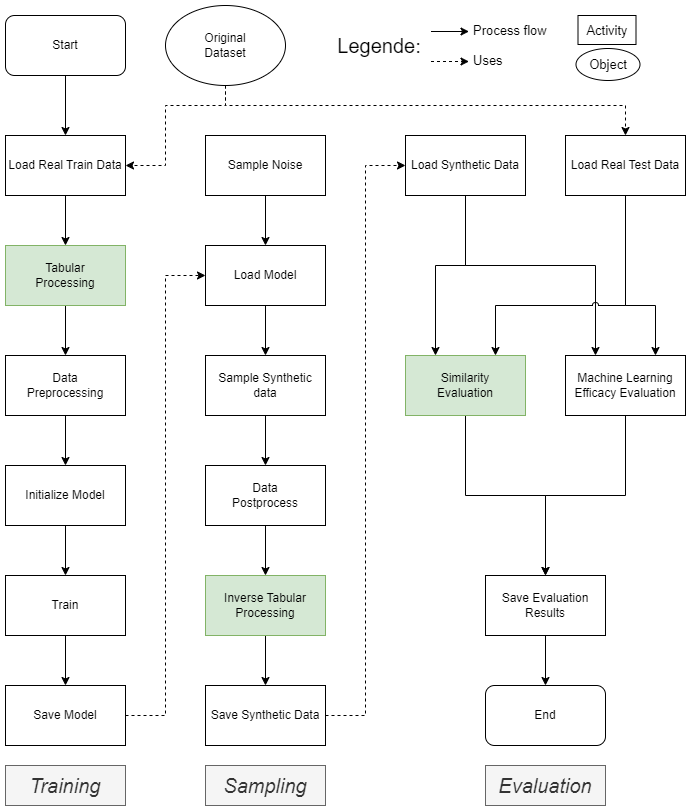
\includegraphics[width=0.8\textwidth]{images/Overall_changed.png}
    \caption{Overview of proposed synthetic data generation process changes (highlighted in green)}
    \label{fig:Overall_changed}
\end{figure}

\begin{description}
    \item[C1-Tabular Processing:] In order to test the effect of different tabular processing techniques, a "Tabular processing" step is required before the training of the diffusion model.
    Within this processing, the raw data is transformed according to the defined tabular processing strategy.
    The data output format of the tabular processing needs to be in the same like it was before the transformation, which is described in \autoref{sec:data_format}, in order to ensure, 
    that the remain pipeline remains functional and keep changes to the original code minimal.
    \item[C2-Inverse Tabular Processing:] Similar to the data preprocessing, which requires an inverse data postprocessing, to turn the data back into its original format and scale, the same is necessary for the tabular processing.
    Since the model is trained on data that has been transformed according to the tabular processing mechanism, the diffusion model will produce data in the same format.
    Consequently, the synthetic data needs to be transformed back by an inverse function of the tabular processing mechanism used before the training.
    \item[C3-Similarity Evaluation:] Lastly, an extended evaluation on the similarity of the synthetic data compared to the real data should be performed.
    For this, the original evaluation is extended by a similarity score metric, that does not only calculate a unified score, for which the hyperparameters can be tuned towards,
    but also reports other metric results, that are of interests.
    In a addition to the quantitative metric results, several visualization comparing real and synthetic data should be generated, for a qualitative evaluation.
\end{description}



\subsection{Tabular Processing}
\label{ch:conceptualDesign-codeExtensions-dataPreprocessing}

The main source for finding the processing mechanisms should be academic literature, where said mechanism has been applied to a related problem successful
The selection of which tabular processing mechanisms are realized is heavily dependent on the requirements defined in \autoref{sec:func_requirements} (specifically, FR[TODO] - FR[TODO]).

For a tabular processing mechanism to be used, the following conditions must be met:

\begin{enumerate}
    \item reversibility: the tabular processing mechanism must be able to not only transform the data into a different format, it also must be able to revert the transformation,
    such that the data can be transform back into its original form.
    \item compatibility: the data must be able to be separated into numerical and categorical parts after the transformation,
    since the remaining code expects data in this format, as specified in \autoref{sec:data_format}.
    \item complexity: the time it takes for transforming the data should be within a reasonable timeframe, do not add too much additional computation time on the already extensive model tuning process.
    \item availability: due to the limited time frame of this thesis, the code for the mechanisms should be publicly available (or could be implemented within a reasonable timeframe).
\end{enumerate}

based upon the above mentioned criteria, tabular processing mechanisms should be selected.

\section{Experiments}
\label{ch:conceptualDesign-Experiments}

To systematically analyze the performance of the different tabular processing mechanism, the following baseline experiments should be performed:

\begin{description}
    \item[Baseline-Real:] Comparison of the real training data with the real test data. 
    The similarity evaluation is expected to be very high, since the data is from the same distribution.
    The computed machine learning efficacy score can be seen as an objective value that should be reached.
    The closer the synthetic data based machine learning efficacy results are to this target, the better the synthetic data.
    \item[Baseline-TabDDPM:] Reproduction of the TabDDPM results of the authors \cite{kotelnikov2022TabDDPMModellingTabular} but with the addition of computing the similarity evaluation.
    \item[Baseline-TVAE:] Like Baseline-TabDDPM but for TVAE.
    \item[Baseline-CTABGAN:] Like Baseline-TabDDPM but for CTABGAN.
    \item[Baseline-CTABGAN+:] Like Baseline-TabDDPM but for CTABGAN+.
    \item[Baseline-SMOTE:] Like Baseline-TabDDPM but for SMOTE.
\end{description}

For each implemented Tabular Processing mechanism, the following two experiments should be at least performed:

\begin{description}
    \item[Experiment 1:] Tabular Processing combined with TabDDPM with additional similarity evaluation. Hyperparameters tuned like in the original experiment (tuned after CatBoost-machine learning efficacy score).
    \item[Experiment 2:] Like Experiment 1, but hyperparameters are optimized towards the similarity evaluation instead of the machine learning efficacy score.
\end{description}

depending on the results of the above experiments, additional experiments can be performed for a subset of promising Tabular Processing mechanisms, \eg testing different preprocessing methods after the tabular processing.

\subsection[]{Evaluation}
\label{ch:conceptualDesign-Evaluation}
TODO:
ML efficacy like in the original paper + Tabsyndex similarity score + similarity score of anderes paper (+bilder von denen)

aufzählen was alles klassische ml efficacy is (acc, f1, roc) und was sim_score werte sind